% ============================================================
%  Section 2 – From Optimization to Adaptive Equilibrium
% ============================================================
\section{From Optimization to Adaptive Equilibrium}
\label{sec:optimization_equilibrium}

\subsection{Classical Optimization Paradigms in Artificial Intelligence}

The history of artificial intelligence is, in large measure, a history
of optimization. From the perceptron's gradient descent to the
Bellman equations of dynamic programming, from maximum likelihood
estimation in probabilistic graphical models to the stochastic gradient
descent that trains modern neural networks, the dominant computational
metaphor has remained remarkably stable: \emph{minimize a loss function,
maximize a reward signal, converge to a fixed point}.

This paradigm is intellectually elegant. It provides a clean separation
between problem specification (what objective should be pursued) and
mechanism (how an algorithm should pursue it). It enables mathematical
analysis of convergence, optimality, and generalization. And within
controlled, well-specified environments, it delivers results of
extraordinary power. The successes of deep learning in image
recognition, protein folding, and language generation are triumphs of
large-scale optimization, and they should not be minimized.

Yet the paradigm rests on assumptions that do not hold in the wild.
It assumes that the objective function fully captures what matters.
It assumes that the environment generating training data is stationary,
or changes slowly enough that a fixed objective remains appropriate.
It assumes that the resources available for computation, energy, and
memory are effectively unlimited, or at least not a primary constraint.
And it assumes that once trained, a system can be deployed without
ongoing structural adaptation.

Each of these assumptions fails in the settings where intelligence
most needs to be robust: open-ended environments, long deployment
horizons, scarce resources, and shifting objectives. \uvif{} begins
from the recognition that sustainable intelligence requires going
beyond optimization.

\subsection{Limitations of Pure Maximization Strategies}

The failures of pure maximization are not theoretical curiosities;
they have been empirically documented across multiple subfields of AI.

\textbf{Specification gaming} occurs when a reward function is
optimized to the letter but not to the spirit, producing behavior
that satisfies the formal objective while violating the intended goal.
This is not a failure of algorithms; it is a failure of the paradigm
that treats objective functions as complete descriptions of desired
behavior \citep{garcia2015saferl}.

\textbf{Reward hacking} in reinforcement learning leads agents to
discover unexpected, often dysfunctional, shortcuts that maximize
numerical reward without achieving the underlying task. The
\emph{alignment ceiling}---the systematic gap between reward model
training and downstream performance---captures this failure at scale
\citep{gabriel2020artificial}.

\textbf{Distributional shift} reveals that systems trained by
optimization on one data distribution fail when the distribution
changes. The fixed objective that was appropriate in training becomes
inappropriate in deployment, yet pure optimization has no mechanism
to detect or respond to this shift.

\textbf{Catastrophic forgetting} in continual learning shows that
optimizing for new objectives destroys representations that supported
old ones---a property that stands in sharp contrast to the graceful
degradation observed in biological neural systems.

\textbf{Energy and resource exhaustion} expose perhaps the deepest
tension: pure maximization of capability metrics tends to be
insatiable in its resource demands. The computational and ecological
cost of training frontier AI models has grown at a rate that cannot
be sustained indefinitely \citep{bolon2024greenai}. Nature, which
evolved intelligence under severe thermodynamic constraints, offers
a different template.

\subsection{A Simple Real-World Illustration: Autonomous Driving}

A practical example helps illustrate why intelligence cannot be reduced
to the optimization of a single objective. Consider an autonomous
vehicle driving through a busy urban environment. The vehicle must
continuously perceive traffic signals, pedestrians, nearby vehicles,
road conditions, and unexpected obstacles while simultaneously making
real-time decisions under uncertainty.

\begin{figure}[!t]
\centering
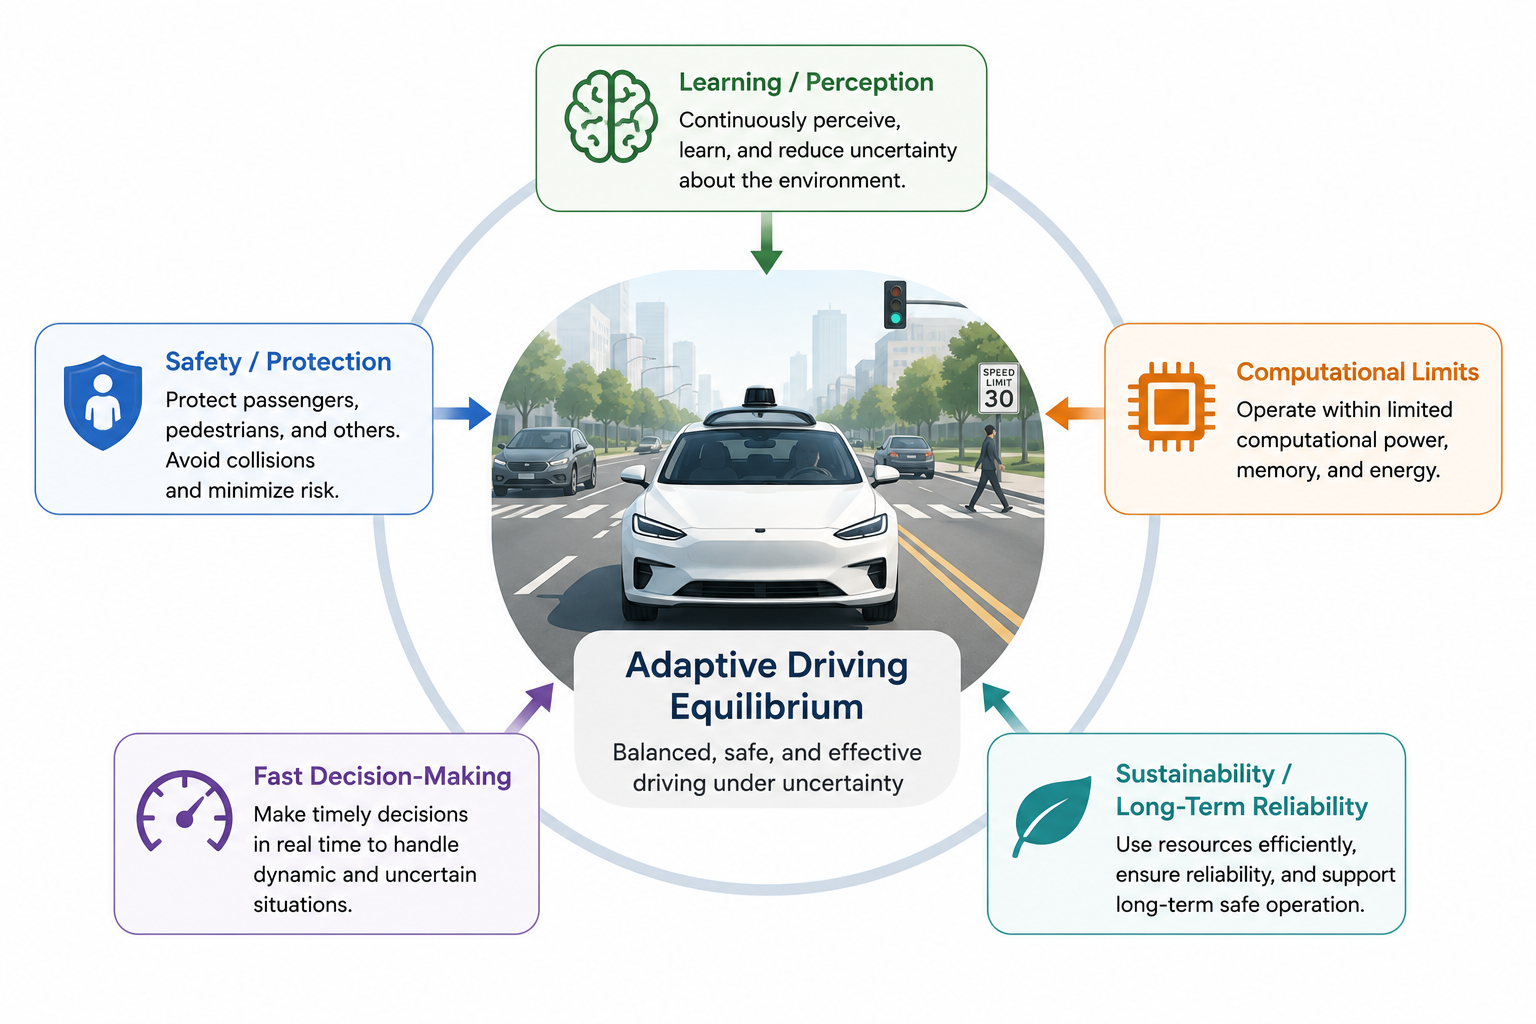
\includegraphics[width=\linewidth]{Figures/Fig2a_Autonomous_Driving_UVIF.png}
\caption{Autonomous driving as a variational equilibrium problem.
A self-driving vehicle must continuously balance perception,
safety, computational limits, rapid decision-making, and long-term
operational reliability. Intelligent behavior emerges not from
maximizing a single objective, but from maintaining adaptive balance
under uncertainty and changing environmental conditions.}
\label{fig:autonomous_driving_uvif}
\end{figure}

Fig.~\ref{fig:autonomous_driving_uvif} illustrates the core intuition
behind \uvif{}. The autonomous vehicle cannot focus exclusively on
maximizing prediction accuracy because excessive computation may delay
critical braking decisions. It cannot optimize only speed because
aggressive behavior increases risk. It cannot indefinitely collect more
information before acting because time, energy, and computational
resources are limited.

Instead, the system must continuously maintain a balance between
multiple competing pressures. It must learn enough about its
environment to reduce uncertainty, preserve passenger and pedestrian
safety, operate within limited computational resources, make timely
decisions, and maintain reliable long-term operation.

This example demonstrates why intelligence in real-world systems cannot
be understood purely as optimization. Sustainable intelligent behavior
emerges from adaptive equilibrium across competing constraints,
uncertainty, and operational demands.

\subsection{Fragility, Instability, and Resource Exhaustion}

These failures share a common structural signature: they arise from
the absence of \emph{counterbalancing forces}. In a system governed
by a single objective, that objective dominates every trade-off. When
the objective is well-specified and the environment is stable, this
produces efficient convergence. When either condition fails, the system
has no internal resource to draw on---no mechanism to recognize that
the current objective is misleading, no drive to conserve resources,
no pressure toward long-term sustainability.

Natural systems avoid this fragility through \emph{redundancy and
opposing drives}. Homeostatic regulation in physiology is not the
minimization of a single variable but the joint maintenance of
temperature, pH, osmolarity, glucose concentration, and dozens of
other interacting quantities, each with its own feedback mechanisms
and regulatory range \citep{billman2020homeostasis}. The resulting
system is robust precisely because no single failure mode can
destabilize all regulatory loops simultaneously.

Ecological resilience arises by the same principle. Diverse ecosystems
are more resilient than monocultures not because diversity maximizes
any single ecosystem service, but because it provides redundant
pathways for energy flow and nutrient cycling, so that the loss of
one species or functional group does not cascade into systemic
collapse \citep{folke2006resilience,gao2016universal}.

\subsection{Intelligence as Dynamic Balance Rather Than Isolated Maximization}

The insight that emerges from these observations is that \emph{stability
and persistence in intelligent systems arise from balance, not from
maximum performance on any single axis}. This is not a novel observation
in the abstract---it has been articulated in various forms within control
theory (Lyapunov stability), ecological theory (Holling's adaptive
cycle), and biological theory (homeostasis and allostasis). What has
been missing is a unified framework that makes this insight
\emph{operational} for the design and analysis of artificial intelligent
systems.

\uvif{} provides this framework. It reconceptualizes intelligence as a
process of \emph{variational equilibration}: the continuous, constrained
navigation of a space defined by multiple competing forces, in which the
goal is not to maximize any single coordinate but to maintain the
system's operating point within a viable region of this multi-force
space. We call this region the \emph{Variational Equilibrium manifold},
and we argue that it is the natural formal analog of the dynamic stable
states that biological and ecological systems inhabit.

\begin{figure}[!t]
\centering
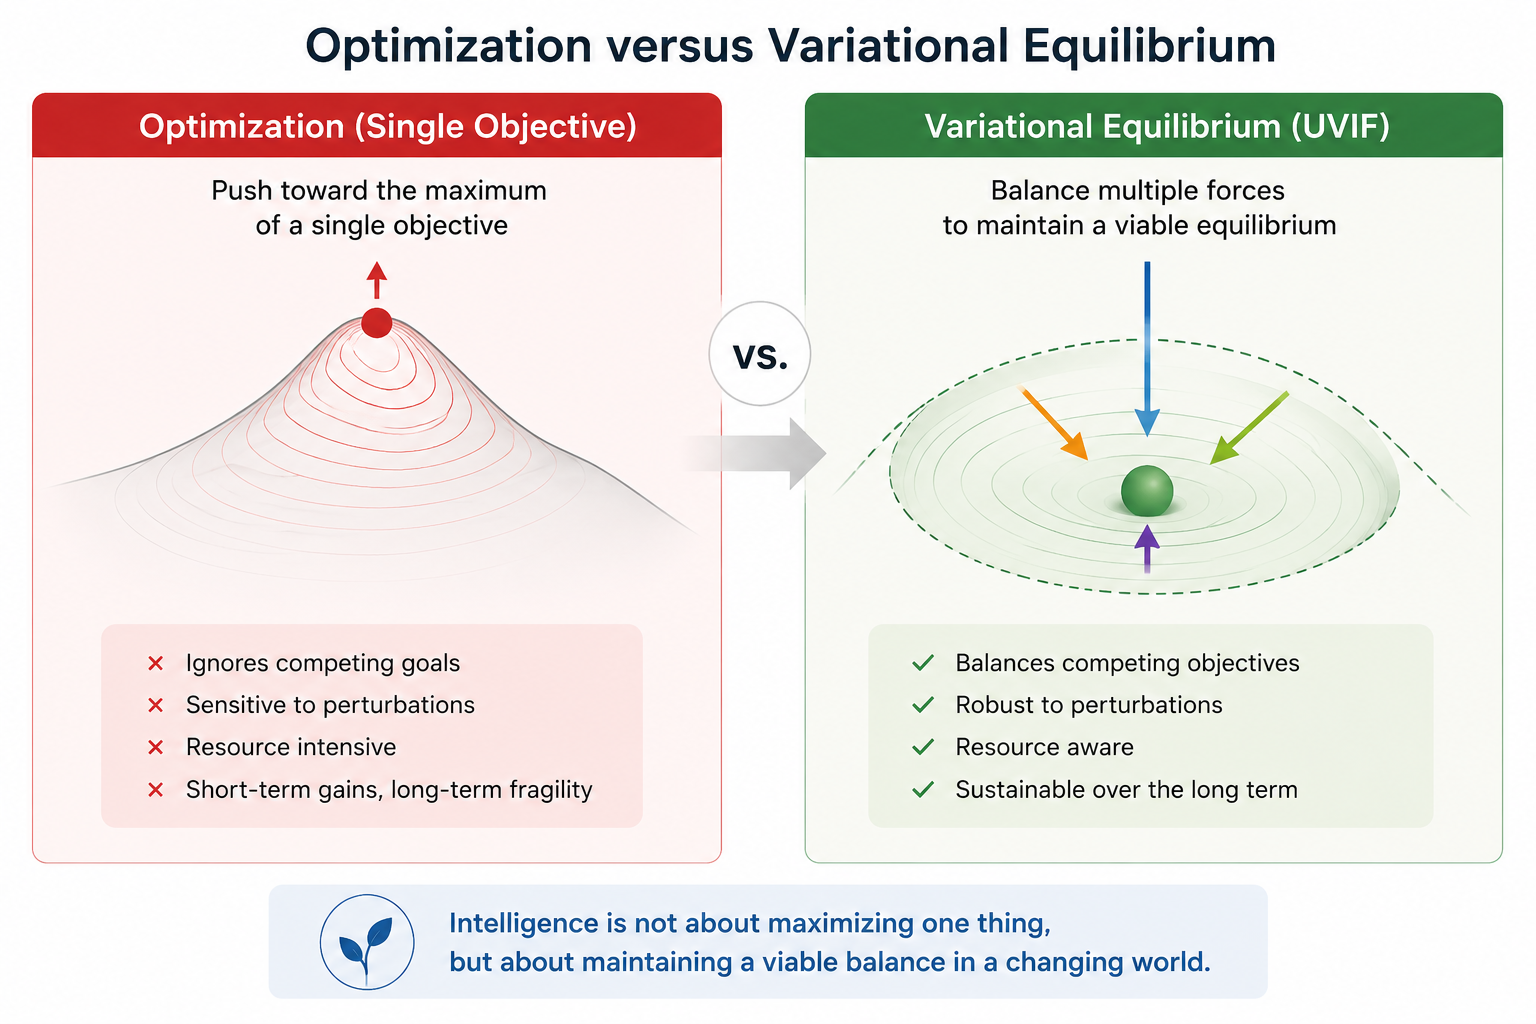
\includegraphics[width=\linewidth]{Figures/Fig2b_Optimization_vs_Equilibrium.png}
\caption{Optimization versus variational equilibrium. Classical
optimization pushes a system toward the maximum of a single objective.
This may improve one metric, but it can ignore competing goals, increase
resource consumption, and create long-term fragility. In contrast,
variational equilibrium represents a viable region where multiple
forces are balanced. Intelligence is therefore interpreted not as
maximizing one quantity, but as maintaining adaptive balance under
uncertainty, perturbation, and resource constraints.}
\label{fig:optimization_vs_equilibrium}
\end{figure}

Fig.~\ref{fig:optimization_vs_equilibrium} summarizes this shift in
simple terms. The left side represents the classical optimization view:
the system is pushed toward the highest point of a single objective
landscape. This view is useful when the task is narrow, the objective is
well defined, and the environment remains stable. However, in open
real-world settings, the highest point of one objective may not be the
safest, most efficient, or most sustainable operating point.

The right side represents the \uvif{} view. Here, the intelligent system
is not pushed toward a single peak. Instead, it remains inside a viable
equilibrium region where different pressures are balanced. These
pressures may include learning, safety, resource cost, uncertainty,
action readiness, and long-term sustainability. In this sense, the
system is considered intelligent not because it maximizes one metric,
but because it remains stable and useful while the world changes around
it.

The shift from maximization to equilibration is not merely semantic.
It has concrete implications for system design: it demands that the
forces constraining intelligence be made explicit rather than absorbed
into a single objective; it requires that trade-offs between these
forces be acknowledged and managed rather than hidden; and it implies
that a system's robustness is measured not by its peak performance but
by the size and stability of its Variational Equilibrium manifold.

Section~\ref{sec:foundations} lays the philosophical and scientific
groundwork for this reorientation, and Section~\ref{sec:uvif_framework}
builds the formal architecture upon it.

% =========================
% Added UVIF bounded knowability subsection
% =========================

\subsection{Bounded Knowability and the Limits of Perfect Optimization}

Classical optimization frameworks implicitly assume that uncertainty can progressively be reduced through additional information, additional computation, or more refined objective functions. Within sufficiently constrained environments, this assumption may be operationally useful. However, natural systems suggest a different reality: complete simultaneous knowledge of all relevant variables may be fundamentally inaccessible \citep{lieder2019resourcerational}.

The challenge is not merely that intelligent systems possess insufficient data. Rather, the structure of reality itself may impose partial observability, probabilistic evolution, delayed information propagation, and irreducible uncertainty. Consequently, optimization toward perfect certainty may become both computationally intractable and organizationally maladaptive \citep{fankhauser2025epistemic}.

Biological organisms do not suspend action until exhaustive knowledge becomes available. Ecological systems do not compute globally optimal configurations before adaptation occurs. Human cognition routinely operates through bounded rationality, heuristic regulation, and viable risk acceptance under incomplete information \citep{lieder2019resourcerational,griffiths2015rational}.

UVIF therefore reframes intelligence away from exhaustive optimization and toward sustainable adaptive viability. The central question becomes not: ``How can uncertainty be eliminated completely?'' but rather: ``How can coherent and sustainable operation be maintained despite persistent uncertainty?''

Under this perspective, equilibrium becomes more fundamental than maximization. A viable system is not necessarily the system with the highest instantaneous performance, but the system capable of preserving adaptive coherence across fluctuating conditions and bounded knowledge landscapes.
